\subsection*{Teil B: Symmetrie erkennen (20 Minuten)}

\begin{enumerate}[label=\arabic*.]
    \item \textbf{Welche Figuren sind achsensymmetrisch? Kreuze an und zeichne die Symmetrieachsen ein:}
    \vspace{0.5cm}

    \begin{tabular}{|l|c|c|}
        \hline
        \textbf{Figur} & \textbf{Achsensymmetrisch?} & \textbf{Anzahl Symmetrieachsen} \\
        \hline
        Rechteck & $\square$ Ja $\square$ Nein & \underline{\hspace{2cm}} \\
        \hline
        Gleichseitiges Dreieck & $\square$ Ja $\square$ Nein & \underline{\hspace{2cm}} \\
        \hline
        Parallelogramm & $\square$ Ja $\square$ Nein & \underline{\hspace{2cm}} \\
        \hline
        Quadrat & $\square$ Ja $\square$ Nein & \underline{\hspace{2cm}} \\
        \hline
        Kreis & $\square$ Ja $\square$ Nein & \underline{\hspace{2cm}} \\
        \hline
    \end{tabular}

    \vspace{1cm}

    \item \textbf{Zeichne die Symmetrieachsen in diese Figuren ein:}
    \vspace{0.5cm}

    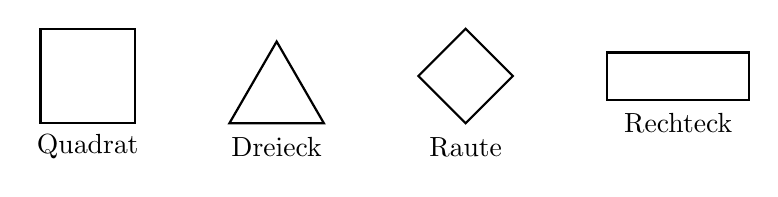
\begin{tikzpicture}[scale=0.6]
        % Quadrat
        \draw[thick] (0,0) rectangle (2,2);
        \node at (1,-0.5) {Quadrat};

        % Gleichseitiges Dreieck
        \draw[thick] (4,0) -- (6,0) -- (5,1.73) -- cycle;
        \node at (5,-0.5) {Dreieck};

        % Raute
        \draw[thick] (8,1) -- (9,2) -- (10,1) -- (9,0) -- cycle;
        \node at (9,-0.5) {Raute};

        % Rechteck
        \draw[thick] (12,0.5) rectangle (15,1.5);
        \node at (13.5,-0) {Rechteck};
    \end{tikzpicture}
\end{enumerate}